\documentclass[twoside]{book}

% Packages required by doxygen
\usepackage{fixltx2e}
\usepackage{calc}
\usepackage{doxygen}
\usepackage[export]{adjustbox} % also loads graphicx
\usepackage{graphicx}
\usepackage[utf8]{inputenc}
\usepackage{makeidx}
\usepackage{multicol}
\usepackage{multirow}
\PassOptionsToPackage{warn}{textcomp}
\usepackage{textcomp}
\usepackage[nointegrals]{wasysym}
\usepackage[table]{xcolor}

% Font selection
\usepackage[T1]{fontenc}
\usepackage[scaled=.90]{helvet}
\usepackage{courier}
\usepackage{amssymb}
\usepackage{sectsty}
\renewcommand{\familydefault}{\sfdefault}
\allsectionsfont{%
  \fontseries{bc}\selectfont%
  \color{darkgray}%
}
\renewcommand{\DoxyLabelFont}{%
  \fontseries{bc}\selectfont%
  \color{darkgray}%
}
\newcommand{\+}{\discretionary{\mbox{\scriptsize$\hookleftarrow$}}{}{}}

% Page & text layout
\usepackage{geometry}
\geometry{%
  a4paper,%
  top=2.5cm,%
  bottom=2.5cm,%
  left=2.5cm,%
  right=2.5cm%
}
\tolerance=750
\hfuzz=15pt
\hbadness=750
\setlength{\emergencystretch}{15pt}
\setlength{\parindent}{0cm}
\setlength{\parskip}{3ex plus 2ex minus 2ex}
\makeatletter
\renewcommand{\paragraph}{%
  \@startsection{paragraph}{4}{0ex}{-1.0ex}{1.0ex}{%
    \normalfont\normalsize\bfseries\SS@parafont%
  }%
}
\renewcommand{\subparagraph}{%
  \@startsection{subparagraph}{5}{0ex}{-1.0ex}{1.0ex}{%
    \normalfont\normalsize\bfseries\SS@subparafont%
  }%
}
\makeatother

% Headers & footers
\usepackage{fancyhdr}
\pagestyle{fancyplain}
\fancyhead[LE]{\fancyplain{}{\bfseries\thepage}}
\fancyhead[CE]{\fancyplain{}{}}
\fancyhead[RE]{\fancyplain{}{\bfseries\leftmark}}
\fancyhead[LO]{\fancyplain{}{\bfseries\rightmark}}
\fancyhead[CO]{\fancyplain{}{}}
\fancyhead[RO]{\fancyplain{}{\bfseries\thepage}}
\fancyfoot[LE]{\fancyplain{}{}}
\fancyfoot[CE]{\fancyplain{}{}}
\fancyfoot[RE]{\fancyplain{}{\bfseries\scriptsize Generated by Doxygen }}
\fancyfoot[LO]{\fancyplain{}{\bfseries\scriptsize Generated by Doxygen }}
\fancyfoot[CO]{\fancyplain{}{}}
\fancyfoot[RO]{\fancyplain{}{}}
\renewcommand{\footrulewidth}{0.4pt}
\renewcommand{\chaptermark}[1]{%
  \markboth{#1}{}%
}
\renewcommand{\sectionmark}[1]{%
  \markright{\thesection\ #1}%
}

% Indices & bibliography
\usepackage{natbib}
\usepackage[titles]{tocloft}
\setcounter{tocdepth}{3}
\setcounter{secnumdepth}{5}
\makeindex

% Custom commands
\newcommand{\clearemptydoublepage}{%
  \newpage{\pagestyle{empty}\cleardoublepage}%
}

\usepackage{caption}
\captionsetup{labelsep=space,justification=centering,font={bf},singlelinecheck=off,skip=4pt,position=top}

%===== C O N T E N T S =====

\begin{document}

% Titlepage & ToC
\pagenumbering{roman}
\begin{titlepage}
\vspace*{7cm}
\begin{center}%
{\Large P\+H\+P/\+My\+S\+QL A\+PI }\\
\vspace*{1cm}
{\large Generated by Doxygen 1.8.11}\\
\end{center}
\end{titlepage}
\clearemptydoublepage
\tableofcontents
\clearemptydoublepage
\pagenumbering{arabic}

%--- Begin generated contents ---
\chapter{Hierarchical Index}
\section{Class Hierarchy}
This inheritance list is sorted roughly, but not completely, alphabetically\+:\begin{DoxyCompactList}
\item \contentsline{section}{Common\+Interface}{\pageref{interface_common_interface}}{}
\begin{DoxyCompactList}
\item \contentsline{section}{Common}{\pageref{class_common}}{}
\end{DoxyCompactList}
\item \contentsline{section}{D\+B\+Interface}{\pageref{interface_d_b_interface}}{}
\begin{DoxyCompactList}
\item \contentsline{section}{D\+B\+A\+PI}{\pageref{class_d_b_a_p_i}}{}
\end{DoxyCompactList}
\item \contentsline{section}{P\+D\+B\+A\+PI}{\pageref{class_p_d_b_a_p_i_1_1_p_d_b_a_p_i}}{}
\end{DoxyCompactList}

\chapter{Data Structure Index}
\section{Data Structures}
Here are the data structures with brief descriptions\+:\begin{DoxyCompactList}
\item\contentsline{section}{{\bf Common} }{\pageref{class_common}}{}
\item\contentsline{section}{{\bf Common\+Interface} }{\pageref{interface_common_interface}}{}
\item\contentsline{section}{{\bf D\+B\+A\+PI} }{\pageref{class_d_b_a_p_i}}{}
\item\contentsline{section}{{\bf D\+B\+Interface} }{\pageref{interface_d_b_interface}}{}
\item\contentsline{section}{{\bf P\+D\+B\+A\+PI} }{\pageref{class_p_d_b_a_p_i_1_1_p_d_b_a_p_i}}{}
\end{DoxyCompactList}

\chapter{Data Structure Documentation}
\section{Common Class Reference}
\label{class_common}\index{Common@{Common}}
Inheritance diagram for Common\+:\begin{figure}[H]
\begin{center}
\leavevmode
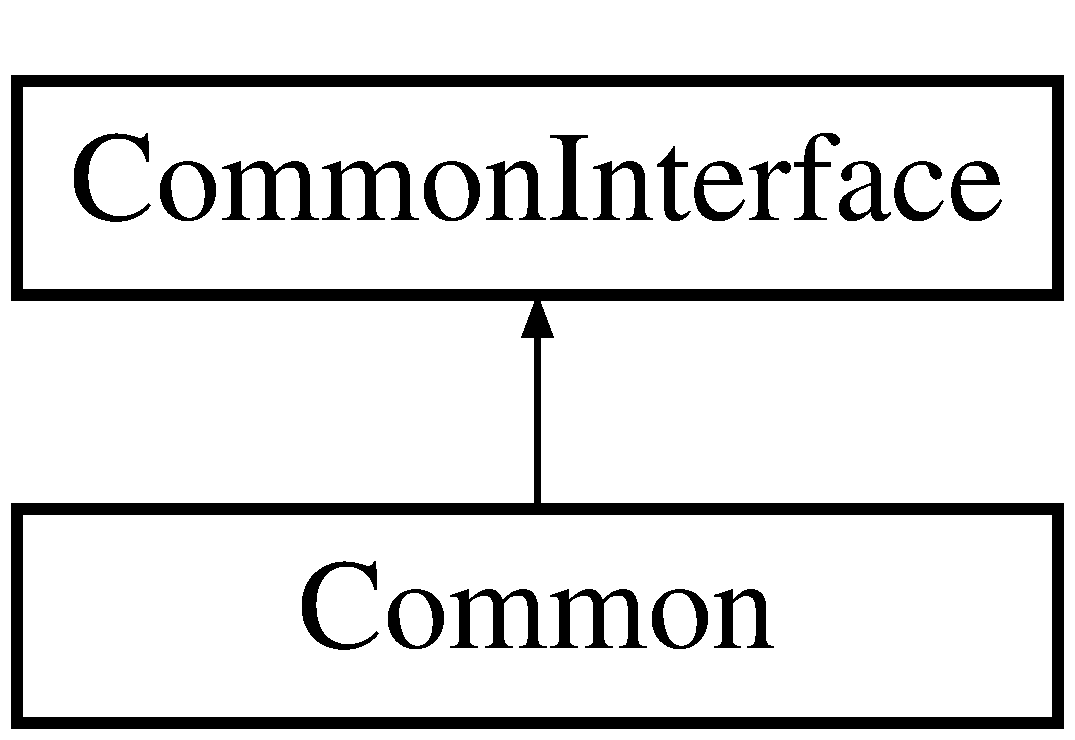
\includegraphics[height=2.000000cm]{class_common}
\end{center}
\end{figure}
\subsection*{Public Member Functions}
\begin{DoxyCompactItemize}
\item 
{\bf Common} (\$debug)
\item 
{\bf connect} (\$db)
\item 
{\bf execute\+Query} (\$sql, \$filename)
\end{DoxyCompactItemize}
\subsection*{Data Fields}
\begin{DoxyCompactItemize}
\item 
{\bf \$conn}
\item 
{\bf \$debug}
\item 
{\bf \$db} =\char`\"{}database.\+cse.\+tamu.\+edu\char`\"{}
\item 
{\bf \$dbname} =\char`\"{}jgwesterfield-\/Walker\+Data\char`\"{}
\item 
{\bf \$user} =\char`\"{}jgwesterfield\char`\"{}
\item 
{\bf \$pass} =\char`\"{}Whoop19!\char`\"{}
\end{DoxyCompactItemize}


\subsection{Detailed Description}
Created by Php\+Storm. User\+: Jonathan\+Westerfield Date\+: 2/8/18 Time\+: 4\+:20 PM 

Definition at line 9 of file Common\+Methods.\+php.



\subsection{Member Function Documentation}
\index{Common@{Common}!Common@{Common}}
\index{Common@{Common}!Common@{Common}}
\subsubsection[{Common(\$debug)}]{\setlength{\rightskip}{0pt plus 5cm}{\bf Common} (
\begin{DoxyParamCaption}
\item[{}]{\$debug}
\end{DoxyParamCaption}
)}\label{class_common_a4a9e6769ab6c946d0895e8d987df1c10}


Implements {\bf Common\+Interface} \doxyref{}{p.}{interface_common_interface_a4a9e6769ab6c946d0895e8d987df1c10}.



Definition at line 25 of file Common\+Methods.\+php.

\index{Common@{Common}!connect@{connect}}
\index{connect@{connect}!Common@{Common}}
\subsubsection[{connect(\$db)}]{\setlength{\rightskip}{0pt plus 5cm}connect (
\begin{DoxyParamCaption}
\item[{}]{\$db}
\end{DoxyParamCaption}
)}\label{class_common_a1b1bd9b3f45a5fbd2549355282cdc96f}


Implements {\bf Common\+Interface} \doxyref{}{p.}{interface_common_interface_a1b1bd9b3f45a5fbd2549355282cdc96f}.



Definition at line 34 of file Common\+Methods.\+php.

\index{Common@{Common}!execute\+Query@{execute\+Query}}
\index{execute\+Query@{execute\+Query}!Common@{Common}}
\subsubsection[{execute\+Query(\$sql, \$filename)}]{\setlength{\rightskip}{0pt plus 5cm}execute\+Query (
\begin{DoxyParamCaption}
\item[{}]{\$sql, }
\item[{}]{\$filename}
\end{DoxyParamCaption}
)}\label{class_common_a57a9dbd1203cf7b3ef3c5ce40d4047cc}


Implements {\bf Common\+Interface} \doxyref{}{p.}{interface_common_interface_a57a9dbd1203cf7b3ef3c5ce40d4047cc}.



Definition at line 49 of file Common\+Methods.\+php.



\subsection{Field Documentation}
\index{Common@{Common}!\$conn@{\$conn}}
\index{\$conn@{\$conn}!Common@{Common}}
\subsubsection[{\$conn}]{\setlength{\rightskip}{0pt plus 5cm}\$conn}\label{class_common_aa8a5a87b9c1a6a0819b88447cbe41877}


Definition at line 11 of file Common\+Methods.\+php.

\index{Common@{Common}!\$db@{\$db}}
\index{\$db@{\$db}!Common@{Common}}
\subsubsection[{\$db}]{\setlength{\rightskip}{0pt plus 5cm}\$db =\char`\"{}database.\+cse.\+tamu.\+edu\char`\"{}}\label{class_common_a1fa3127fc82f96b1436d871ef02be319}


Definition at line 20 of file Common\+Methods.\+php.

\index{Common@{Common}!\$dbname@{\$dbname}}
\index{\$dbname@{\$dbname}!Common@{Common}}
\subsubsection[{\$dbname}]{\setlength{\rightskip}{0pt plus 5cm}\$dbname =\char`\"{}jgwesterfield-\/Walker\+Data\char`\"{}}\label{class_common_ac5111a571fffa2499732833bb7f0d8c1}


Definition at line 21 of file Common\+Methods.\+php.

\index{Common@{Common}!\$debug@{\$debug}}
\index{\$debug@{\$debug}!Common@{Common}}
\subsubsection[{\$debug}]{\setlength{\rightskip}{0pt plus 5cm}\$debug}\label{class_common_a85ae3e64cd40e9564adceb010085e9dd}


Definition at line 12 of file Common\+Methods.\+php.

\index{Common@{Common}!\$pass@{\$pass}}
\index{\$pass@{\$pass}!Common@{Common}}
\subsubsection[{\$pass}]{\setlength{\rightskip}{0pt plus 5cm}\$pass =\char`\"{}Whoop19!\char`\"{}}\label{class_common_a12ec2780b52bd1c54d38c2f981c0349f}


Definition at line 23 of file Common\+Methods.\+php.

\index{Common@{Common}!\$user@{\$user}}
\index{\$user@{\$user}!Common@{Common}}
\subsubsection[{\$user}]{\setlength{\rightskip}{0pt plus 5cm}\$user =\char`\"{}jgwesterfield\char`\"{}}\label{class_common_a598ca4e71b15a1313ec95f0df1027ca5}


Definition at line 22 of file Common\+Methods.\+php.



The documentation for this class was generated from the following file\+:\begin{DoxyCompactItemize}
\item 
Users/\+Jonathan\+Westerfield/\+Documents/\+C\+S\+C\+E 315/\+Rec\+Walker\+Counter/{\bf Common\+Methods.\+php}\end{DoxyCompactItemize}

\section{Common\+Interface Interface Reference}
\label{interface_common_interface}\index{Common\+Interface@{Common\+Interface}}
Inheritance diagram for Common\+Interface\+:\begin{figure}[H]
\begin{center}
\leavevmode
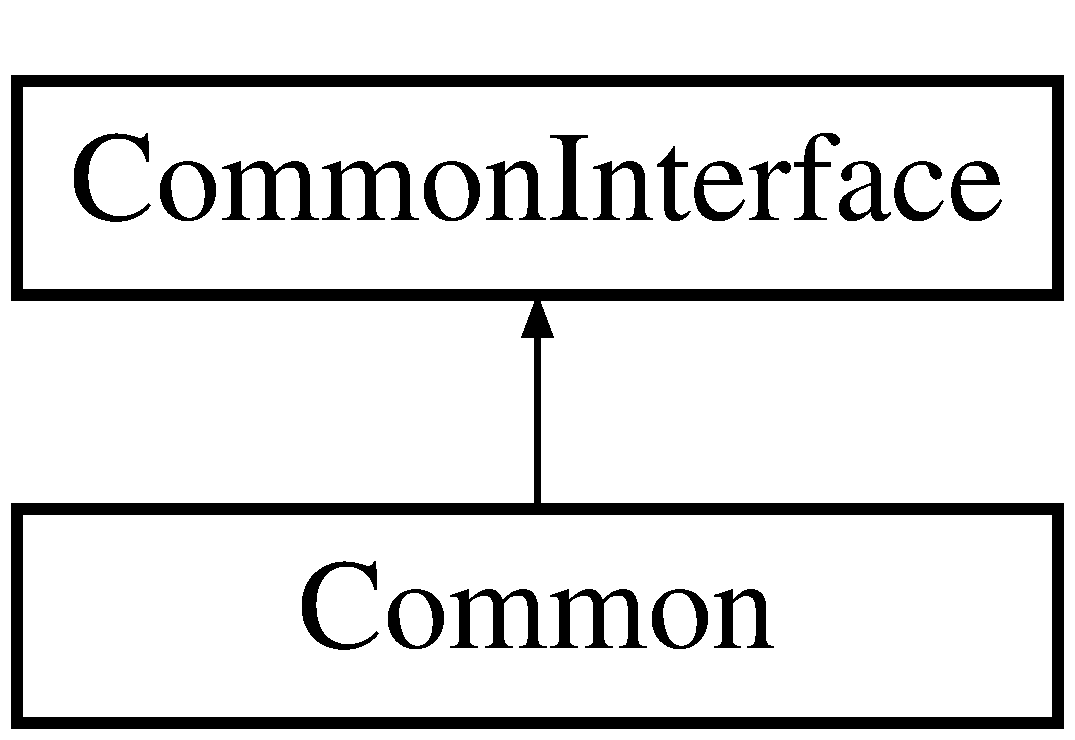
\includegraphics[height=2.000000cm]{interface_common_interface}
\end{center}
\end{figure}
\subsection*{Public Member Functions}
\begin{DoxyCompactItemize}
\item 
{\bfseries Common} (\$debug)\label{interface_common_interface_a4a9e6769ab6c946d0895e8d987df1c10}

\item 
{\bfseries connect} (\$db)\label{interface_common_interface_a1b1bd9b3f45a5fbd2549355282cdc96f}

\item 
{\bfseries execute\+Query} (\$sql, \$filename)\label{interface_common_interface_a57a9dbd1203cf7b3ef3c5ce40d4047cc}

\end{DoxyCompactItemize}


\subsection{Detailed Description}
Created by Php\+Storm. User\+: Jonathan\+Westerfield Date\+: 2/8/18 Time\+: 4\+:31 PM

This is an interface for \doxyref{Common}{p.}{class_common}. 

The documentation for this interface was generated from the following file\+:\begin{DoxyCompactItemize}
\item 
P\+H\+P\+:\+Mysql A\+P\+I/Common\+Interface.\+php\end{DoxyCompactItemize}

\section{D\+B\+A\+PI Class Reference}
\label{class_d_b_a_p_i}\index{D\+B\+A\+PI@{D\+B\+A\+PI}}
Inheritance diagram for D\+B\+A\+PI\+:\begin{figure}[H]
\begin{center}
\leavevmode
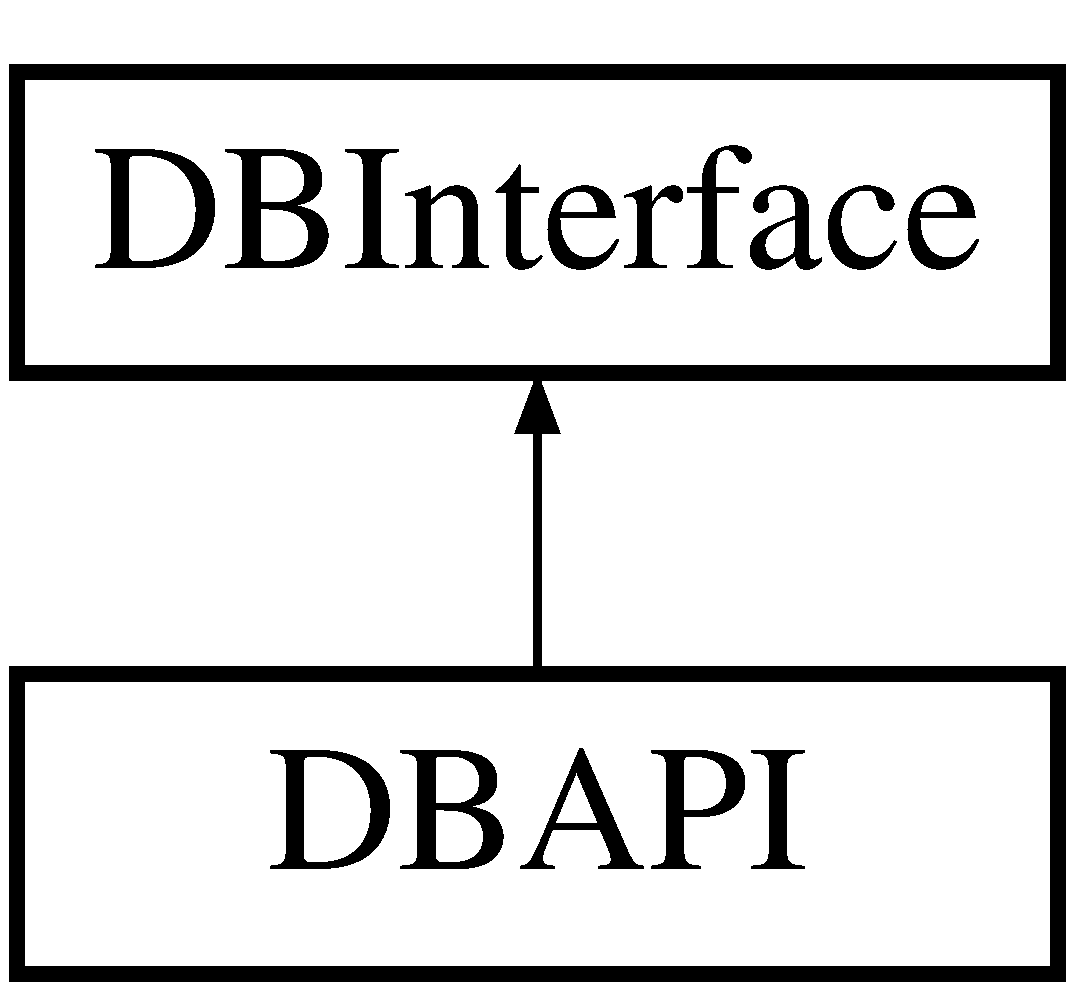
\includegraphics[height=2.000000cm]{class_d_b_a_p_i}
\end{center}
\end{figure}
\subsection*{Public Member Functions}
\begin{DoxyCompactItemize}
\item 
{\bf \+\_\+\+\_\+construct} (\$db)
\item 
{\bf \+\_\+\+\_\+destruct} ()
\item 
{\bf print\+Entire\+DB} ()
\item 
{\bf get\+Total\+Num\+Walkers} ()
\item 
{\bf get\+Num\+Walkers\+Today} ()
\item 
{\bf get\+Num\+Walkers\+This\+Week} ()
\item 
{\bf get\+Current\+Year\+Traffic} ()
\item 
{\bf get\+Traffic\+By\+Year} (\$year)
\item 
{\bf get\+Current\+Month\+Traffic} ()
\item 
{\bf get\+Traffic\+By\+Month} (\$year, \$month)
\item 
{\bf get\+Current\+Day\+Traffic} ()
\item 
{\bf get\+Traffic\+By\+Day} (\$year, \$month, \$day)
\item 
{\bf get\+Traffic\+Time\+Range} (\$year1, \$month1, \$day1, \$year2, \$month2, \$day2)
\end{DoxyCompactItemize}


\subsection{Detailed Description}
Created by Php\+Storm. User\+: Jonathan\+Westerfield Date\+: 2/8/18 Time\+: 4\+:35 PM

Includes the various functions that can be used in order to extract useful information from the database. Implements D\+B\+Interface.\+php 

\subsection{Constructor \& Destructor Documentation}
\index{D\+B\+A\+PI@{D\+B\+A\+PI}!\+\_\+\+\_\+construct@{\+\_\+\+\_\+construct}}
\index{\+\_\+\+\_\+construct@{\+\_\+\+\_\+construct}!D\+B\+A\+PI@{D\+B\+A\+PI}}
\subsubsection[{\+\_\+\+\_\+construct(\$db)}]{\setlength{\rightskip}{0pt plus 5cm}\+\_\+\+\_\+construct (
\begin{DoxyParamCaption}
\item[{}]{\$db}
\end{DoxyParamCaption}
)}\label{class_d_b_a_p_i_a800f8efee13692788b13ee57c5960092}
\doxyref{D\+B\+A\+PI}{p.}{class_d_b_a_p_i} constructor. 
\begin{DoxyParams}{Parameters}
{\em \$db} & Mostly sets up the dates in this object. Also sets the timezone to our timezone. \\
\hline
\end{DoxyParams}


Implements {\bf D\+B\+Interface} \doxyref{}{p.}{interface_d_b_interface_a800f8efee13692788b13ee57c5960092}.

\index{D\+B\+A\+PI@{D\+B\+A\+PI}!\+\_\+\+\_\+destruct@{\+\_\+\+\_\+destruct}}
\index{\+\_\+\+\_\+destruct@{\+\_\+\+\_\+destruct}!D\+B\+A\+PI@{D\+B\+A\+PI}}
\subsubsection[{\+\_\+\+\_\+destruct()}]{\setlength{\rightskip}{0pt plus 5cm}\+\_\+\+\_\+destruct (
\begin{DoxyParamCaption}
{}
\end{DoxyParamCaption}
)}\label{class_d_b_a_p_i_a421831a265621325e1fdd19aace0c758}
Class destructor 

Implements {\bf D\+B\+Interface} \doxyref{}{p.}{interface_d_b_interface}.



\subsection{Member Function Documentation}
\index{D\+B\+A\+PI@{D\+B\+A\+PI}!get\+Current\+Day\+Traffic@{get\+Current\+Day\+Traffic}}
\index{get\+Current\+Day\+Traffic@{get\+Current\+Day\+Traffic}!D\+B\+A\+PI@{D\+B\+A\+PI}}
\subsubsection[{get\+Current\+Day\+Traffic()}]{\setlength{\rightskip}{0pt plus 5cm}get\+Current\+Day\+Traffic (
\begin{DoxyParamCaption}
{}
\end{DoxyParamCaption}
)}\label{class_d_b_a_p_i_a50aa5202dd6a6314b4b0da6fd3026415}
\begin{DoxyReturn}{Returns}
array
\end{DoxyReturn}
Gets the number of people for every hour and returns a length 24 array output the times to see if I overshot how many times to iterate 

Implements {\bf D\+B\+Interface} \doxyref{}{p.}{interface_d_b_interface_a50aa5202dd6a6314b4b0da6fd3026415}.

\index{D\+B\+A\+PI@{D\+B\+A\+PI}!get\+Current\+Month\+Traffic@{get\+Current\+Month\+Traffic}}
\index{get\+Current\+Month\+Traffic@{get\+Current\+Month\+Traffic}!D\+B\+A\+PI@{D\+B\+A\+PI}}
\subsubsection[{get\+Current\+Month\+Traffic()}]{\setlength{\rightskip}{0pt plus 5cm}get\+Current\+Month\+Traffic (
\begin{DoxyParamCaption}
{}
\end{DoxyParamCaption}
)}\label{class_d_b_a_p_i_ae1b5c3c8112356b5c8ea9184286ec89a}
\begin{DoxyReturn}{Returns}
array
\end{DoxyReturn}
Gets the traffic numbers for each day during the current month. 

Implements {\bf D\+B\+Interface} \doxyref{}{p.}{interface_d_b_interface_ae1b5c3c8112356b5c8ea9184286ec89a}.

\index{D\+B\+A\+PI@{D\+B\+A\+PI}!get\+Current\+Year\+Traffic@{get\+Current\+Year\+Traffic}}
\index{get\+Current\+Year\+Traffic@{get\+Current\+Year\+Traffic}!D\+B\+A\+PI@{D\+B\+A\+PI}}
\subsubsection[{get\+Current\+Year\+Traffic()}]{\setlength{\rightskip}{0pt plus 5cm}get\+Current\+Year\+Traffic (
\begin{DoxyParamCaption}
{}
\end{DoxyParamCaption}
)}\label{class_d_b_a_p_i_ad487abf76c66536778a43009612b6843}
\begin{DoxyReturn}{Returns}
array
\end{DoxyReturn}
Returns an array of the traffic numbers for each month in a 12 element array 

Implements {\bf D\+B\+Interface} \doxyref{}{p.}{interface_d_b_interface_ad487abf76c66536778a43009612b6843}.

\index{D\+B\+A\+PI@{D\+B\+A\+PI}!get\+Num\+Walkers\+This\+Week@{get\+Num\+Walkers\+This\+Week}}
\index{get\+Num\+Walkers\+This\+Week@{get\+Num\+Walkers\+This\+Week}!D\+B\+A\+PI@{D\+B\+A\+PI}}
\subsubsection[{get\+Num\+Walkers\+This\+Week()}]{\setlength{\rightskip}{0pt plus 5cm}get\+Num\+Walkers\+This\+Week (
\begin{DoxyParamCaption}
{}
\end{DoxyParamCaption}
)}\label{class_d_b_a_p_i_ae7a2342889cfd984513ba17ddbd14bef}
\begin{DoxyReturn}{Returns}
int
\end{DoxyReturn}
Gets the number of walkers in the last week starting from today 

Implements {\bf D\+B\+Interface} \doxyref{}{p.}{interface_d_b_interface_ae7a2342889cfd984513ba17ddbd14bef}.

\index{D\+B\+A\+PI@{D\+B\+A\+PI}!get\+Num\+Walkers\+Today@{get\+Num\+Walkers\+Today}}
\index{get\+Num\+Walkers\+Today@{get\+Num\+Walkers\+Today}!D\+B\+A\+PI@{D\+B\+A\+PI}}
\subsubsection[{get\+Num\+Walkers\+Today()}]{\setlength{\rightskip}{0pt plus 5cm}get\+Num\+Walkers\+Today (
\begin{DoxyParamCaption}
{}
\end{DoxyParamCaption}
)}\label{class_d_b_a_p_i_adf40141a9763141c0eaeb9ce620181ad}
\begin{DoxyReturn}{Returns}
int
\end{DoxyReturn}
Gets the number of walkers from Today 

Implements {\bf D\+B\+Interface} \doxyref{}{p.}{interface_d_b_interface_adf40141a9763141c0eaeb9ce620181ad}.

\index{D\+B\+A\+PI@{D\+B\+A\+PI}!get\+Total\+Num\+Walkers@{get\+Total\+Num\+Walkers}}
\index{get\+Total\+Num\+Walkers@{get\+Total\+Num\+Walkers}!D\+B\+A\+PI@{D\+B\+A\+PI}}
\subsubsection[{get\+Total\+Num\+Walkers()}]{\setlength{\rightskip}{0pt plus 5cm}get\+Total\+Num\+Walkers (
\begin{DoxyParamCaption}
{}
\end{DoxyParamCaption}
)}\label{class_d_b_a_p_i_ab7a902c85d04b9973a30b73963cb3270}
\begin{DoxyReturn}{Returns}
int
\end{DoxyReturn}
Gets the total number of walkers in the table 

Implements {\bf D\+B\+Interface} \doxyref{}{p.}{interface_d_b_interface_ab7a902c85d04b9973a30b73963cb3270}.

\index{D\+B\+A\+PI@{D\+B\+A\+PI}!get\+Traffic\+By\+Day@{get\+Traffic\+By\+Day}}
\index{get\+Traffic\+By\+Day@{get\+Traffic\+By\+Day}!D\+B\+A\+PI@{D\+B\+A\+PI}}
\subsubsection[{get\+Traffic\+By\+Day(\$year, \$month, \$day)}]{\setlength{\rightskip}{0pt plus 5cm}get\+Traffic\+By\+Day (
\begin{DoxyParamCaption}
\item[{}]{\$year, }
\item[{}]{\$month, }
\item[{}]{\$day}
\end{DoxyParamCaption}
)}\label{class_d_b_a_p_i_a732a3a52aedfb5dd4b63f7292cb8ec3b}

\begin{DoxyParams}{Parameters}
{\em \$year} & \\
\hline
{\em \$month} & \\
\hline
{\em \$day} & \\
\hline
\end{DoxyParams}
\begin{DoxyReturn}{Returns}
array
\end{DoxyReturn}
Gets the traffic for each hour and returns it in a 24 element array.

Usage\+: $<$var = get\+Traffic\+By\+Day(2018, 2, 15);$>$ for Febraury 15, 2018 output the times to see if I overshot how many times to iterate 

Implements {\bf D\+B\+Interface} \doxyref{}{p.}{interface_d_b_interface_a732a3a52aedfb5dd4b63f7292cb8ec3b}.

\index{D\+B\+A\+PI@{D\+B\+A\+PI}!get\+Traffic\+By\+Month@{get\+Traffic\+By\+Month}}
\index{get\+Traffic\+By\+Month@{get\+Traffic\+By\+Month}!D\+B\+A\+PI@{D\+B\+A\+PI}}
\subsubsection[{get\+Traffic\+By\+Month(\$year, \$month)}]{\setlength{\rightskip}{0pt plus 5cm}get\+Traffic\+By\+Month (
\begin{DoxyParamCaption}
\item[{}]{\$year, }
\item[{}]{\$month}
\end{DoxyParamCaption}
)}\label{class_d_b_a_p_i_a0e954fca184f4b8ac04f51cb0c558def}

\begin{DoxyParams}{Parameters}
{\em \$year} & \\
\hline
{\em \$month} & \\
\hline
\end{DoxyParams}
\begin{DoxyReturn}{Returns}
array
\end{DoxyReturn}
Gets the traffic for each day during the specified month of the specified year

Usage\+: get\+Traffic\+By\+Month(2018, 2); // for February 2018 

Implements {\bf D\+B\+Interface} \doxyref{}{p.}{interface_d_b_interface_a0e954fca184f4b8ac04f51cb0c558def}.

\index{D\+B\+A\+PI@{D\+B\+A\+PI}!get\+Traffic\+By\+Year@{get\+Traffic\+By\+Year}}
\index{get\+Traffic\+By\+Year@{get\+Traffic\+By\+Year}!D\+B\+A\+PI@{D\+B\+A\+PI}}
\subsubsection[{get\+Traffic\+By\+Year(\$year)}]{\setlength{\rightskip}{0pt plus 5cm}get\+Traffic\+By\+Year (
\begin{DoxyParamCaption}
\item[{}]{\$year}
\end{DoxyParamCaption}
)}\label{class_d_b_a_p_i_a82c5e558141dca62c793baf0d1216bc0}

\begin{DoxyParams}{Parameters}
{\em \$year} & \\
\hline
\end{DoxyParams}
\begin{DoxyReturn}{Returns}
array
\end{DoxyReturn}
Gives the traffic for each month in an array for the specified year passed in 

Implements {\bf D\+B\+Interface} \doxyref{}{p.}{interface_d_b_interface_a82c5e558141dca62c793baf0d1216bc0}.

\index{D\+B\+A\+PI@{D\+B\+A\+PI}!get\+Traffic\+Time\+Range@{get\+Traffic\+Time\+Range}}
\index{get\+Traffic\+Time\+Range@{get\+Traffic\+Time\+Range}!D\+B\+A\+PI@{D\+B\+A\+PI}}
\subsubsection[{get\+Traffic\+Time\+Range(\$year1, \$month1, \$day1, \$year2, \$month2, \$day2)}]{\setlength{\rightskip}{0pt plus 5cm}get\+Traffic\+Time\+Range (
\begin{DoxyParamCaption}
\item[{}]{\$year1, }
\item[{}]{\$month1, }
\item[{}]{\$day1, }
\item[{}]{\$year2, }
\item[{}]{\$month2, }
\item[{}]{\$day2}
\end{DoxyParamCaption}
)}\label{class_d_b_a_p_i_a546615c71715e031c6218799e97937ab}

\begin{DoxyParams}{Parameters}
{\em \$year1} & \\
\hline
{\em \$month1} & \\
\hline
{\em \$day1} & \\
\hline
{\em \$year2} & \\
\hline
{\em \$month2} & \\
\hline
{\em \$day2} & \\
\hline
\end{DoxyParams}
\begin{DoxyReturn}{Returns}
int
\end{DoxyReturn}
Takes in a date range (start and end date) and counts the number of walkers in the given range 

Implements {\bf D\+B\+Interface} \doxyref{}{p.}{interface_d_b_interface_a546615c71715e031c6218799e97937ab}.

\index{D\+B\+A\+PI@{D\+B\+A\+PI}!print\+Entire\+DB@{print\+Entire\+DB}}
\index{print\+Entire\+DB@{print\+Entire\+DB}!D\+B\+A\+PI@{D\+B\+A\+PI}}
\subsubsection[{print\+Entire\+D\+B()}]{\setlength{\rightskip}{0pt plus 5cm}print\+Entire\+DB (
\begin{DoxyParamCaption}
{}
\end{DoxyParamCaption}
)}\label{class_d_b_a_p_i_a7e02b55449fecf4bed4ca717f38dafd5}
Prints out a table of the entire database 

Implements {\bf D\+B\+Interface} \doxyref{}{p.}{interface_d_b_interface}.



The documentation for this class was generated from the following file\+:\begin{DoxyCompactItemize}
\item 
P\+H\+P\+:\+Mysql A\+P\+I/D\+B\+A\+P\+I.\+php\end{DoxyCompactItemize}

\section{D\+B\+Interface Interface Reference}
\label{interface_d_b_interface}\index{D\+B\+Interface@{D\+B\+Interface}}
Inheritance diagram for D\+B\+Interface\+:\begin{figure}[H]
\begin{center}
\leavevmode
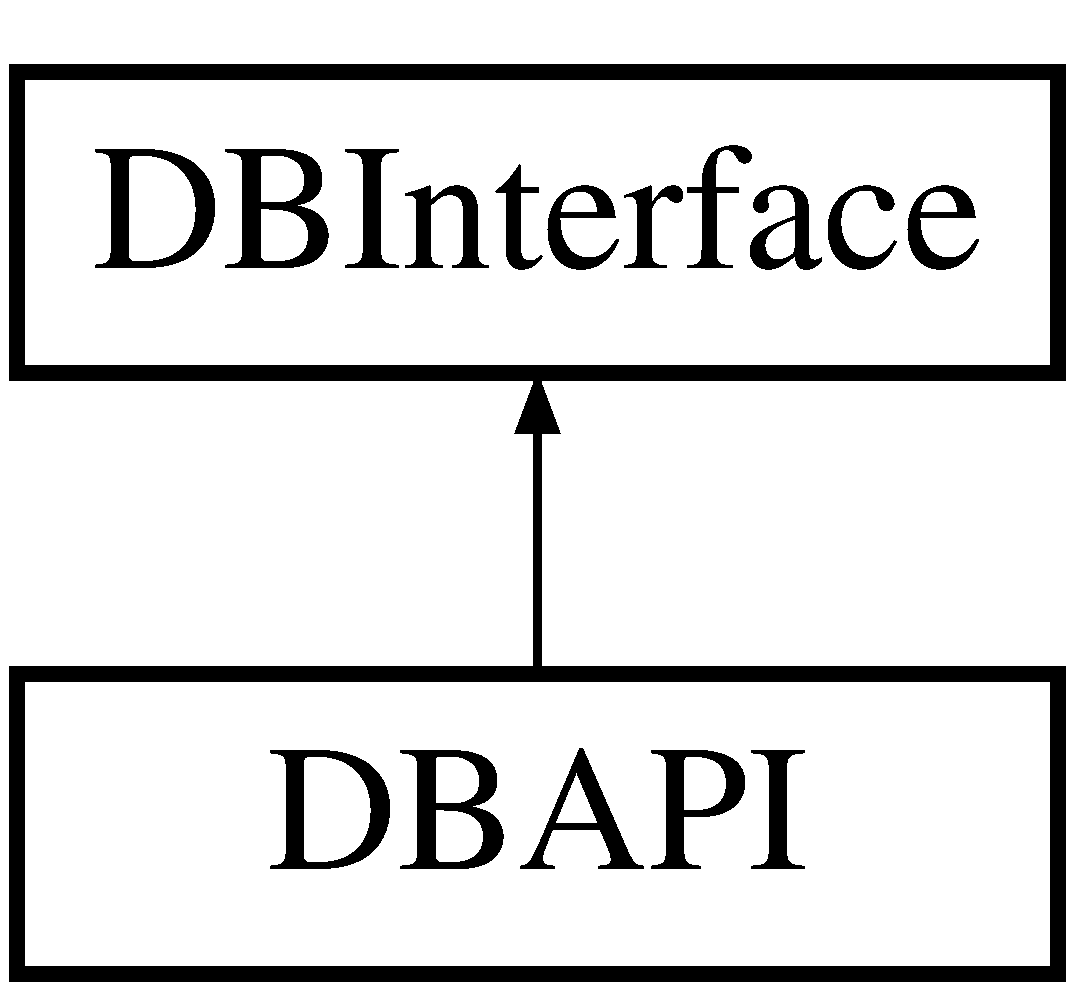
\includegraphics[height=2.000000cm]{interface_d_b_interface}
\end{center}
\end{figure}
\subsection*{Public Member Functions}
\begin{DoxyCompactItemize}
\item 
{\bf \+\_\+\+\_\+construct} (\$db)
\item 
{\bf \+\_\+\+\_\+destruct} ()
\item 
{\bf print\+Entire\+DB} ()
\item 
{\bf get\+Total\+Num\+Walkers} ()
\item 
{\bf get\+Num\+Walkers\+Today} ()
\item 
{\bf get\+Num\+Walkers\+This\+Week} ()
\item 
{\bf get\+Current\+Year\+Traffic} ()
\item 
{\bf get\+Traffic\+By\+Year} (\$year)
\item 
{\bf get\+Current\+Month\+Traffic} ()
\item 
{\bf get\+Traffic\+By\+Month} (\$year, \$month)
\item 
{\bf get\+Current\+Day\+Traffic} ()
\item 
{\bf get\+Traffic\+By\+Day} (\$year, \$month, \$day)
\item 
{\bf get\+Traffic\+Time\+Range} (\$year1, \$month1, \$day1, \$year2, \$month2, \$day2)
\end{DoxyCompactItemize}


\subsection{Detailed Description}
Created by Php\+Storm. User\+: Jonathan\+Westerfield Date\+: 2/8/18 Time\+: 4\+:36 PM 

Definition at line 11 of file D\+B\+Interface.\+php.



\subsection{Constructor \& Destructor Documentation}
\index{D\+B\+Interface@{D\+B\+Interface}!\+\_\+\+\_\+construct@{\+\_\+\+\_\+construct}}
\index{\+\_\+\+\_\+construct@{\+\_\+\+\_\+construct}!D\+B\+Interface@{D\+B\+Interface}}
\subsubsection[{\+\_\+\+\_\+construct(\$db)}]{\setlength{\rightskip}{0pt plus 5cm}\+\_\+\+\_\+construct (
\begin{DoxyParamCaption}
\item[{}]{\$db}
\end{DoxyParamCaption}
)}\label{interface_d_b_interface_a800f8efee13692788b13ee57c5960092}
\doxyref{D\+B\+A\+PI}{p.}{class_d_b_a_p_i} constructor. 
\begin{DoxyParams}{Parameters}
{\em \$db} & Mostly sets up the dates in this object. Also sets the timezone to our timezone. \\
\hline
\end{DoxyParams}


Implemented in {\bf D\+B\+A\+PI} \doxyref{}{p.}{class_d_b_a_p_i_a800f8efee13692788b13ee57c5960092}.

\index{D\+B\+Interface@{D\+B\+Interface}!\+\_\+\+\_\+destruct@{\+\_\+\+\_\+destruct}}
\index{\+\_\+\+\_\+destruct@{\+\_\+\+\_\+destruct}!D\+B\+Interface@{D\+B\+Interface}}
\subsubsection[{\+\_\+\+\_\+destruct()}]{\setlength{\rightskip}{0pt plus 5cm}\+\_\+\+\_\+destruct (
\begin{DoxyParamCaption}
{}
\end{DoxyParamCaption}
)}\label{interface_d_b_interface_a421831a265621325e1fdd19aace0c758}


Implemented in {\bf D\+B\+A\+PI} \doxyref{}{p.}{class_d_b_a_p_i_a421831a265621325e1fdd19aace0c758}.



\subsection{Member Function Documentation}
\index{D\+B\+Interface@{D\+B\+Interface}!get\+Current\+Day\+Traffic@{get\+Current\+Day\+Traffic}}
\index{get\+Current\+Day\+Traffic@{get\+Current\+Day\+Traffic}!D\+B\+Interface@{D\+B\+Interface}}
\subsubsection[{get\+Current\+Day\+Traffic()}]{\setlength{\rightskip}{0pt plus 5cm}get\+Current\+Day\+Traffic (
\begin{DoxyParamCaption}
{}
\end{DoxyParamCaption}
)}\label{interface_d_b_interface_a50aa5202dd6a6314b4b0da6fd3026415}
\begin{DoxyReturn}{Returns}
array
\end{DoxyReturn}
Returns a length 24 array containing total number of walkers for each hour for the current day 

Implemented in {\bf D\+B\+A\+PI} \doxyref{}{p.}{class_d_b_a_p_i_a50aa5202dd6a6314b4b0da6fd3026415}.

\index{D\+B\+Interface@{D\+B\+Interface}!get\+Current\+Month\+Traffic@{get\+Current\+Month\+Traffic}}
\index{get\+Current\+Month\+Traffic@{get\+Current\+Month\+Traffic}!D\+B\+Interface@{D\+B\+Interface}}
\subsubsection[{get\+Current\+Month\+Traffic()}]{\setlength{\rightskip}{0pt plus 5cm}get\+Current\+Month\+Traffic (
\begin{DoxyParamCaption}
{}
\end{DoxyParamCaption}
)}\label{interface_d_b_interface_ae1b5c3c8112356b5c8ea9184286ec89a}
\begin{DoxyReturn}{Returns}
array
\end{DoxyReturn}
Returns an array containing total number of walkers for each day for the current month 

Implemented in {\bf D\+B\+A\+PI} \doxyref{}{p.}{class_d_b_a_p_i_ae1b5c3c8112356b5c8ea9184286ec89a}.

\index{D\+B\+Interface@{D\+B\+Interface}!get\+Current\+Year\+Traffic@{get\+Current\+Year\+Traffic}}
\index{get\+Current\+Year\+Traffic@{get\+Current\+Year\+Traffic}!D\+B\+Interface@{D\+B\+Interface}}
\subsubsection[{get\+Current\+Year\+Traffic()}]{\setlength{\rightskip}{0pt plus 5cm}get\+Current\+Year\+Traffic (
\begin{DoxyParamCaption}
{}
\end{DoxyParamCaption}
)}\label{interface_d_b_interface_ad487abf76c66536778a43009612b6843}
\begin{DoxyReturn}{Returns}
array
\end{DoxyReturn}
Returns an array containing total number of walkers for each month for the current year 12 Element Array 

Implemented in {\bf D\+B\+A\+PI} \doxyref{}{p.}{class_d_b_a_p_i_ad487abf76c66536778a43009612b6843}.

\index{D\+B\+Interface@{D\+B\+Interface}!get\+Num\+Walkers\+This\+Week@{get\+Num\+Walkers\+This\+Week}}
\index{get\+Num\+Walkers\+This\+Week@{get\+Num\+Walkers\+This\+Week}!D\+B\+Interface@{D\+B\+Interface}}
\subsubsection[{get\+Num\+Walkers\+This\+Week()}]{\setlength{\rightskip}{0pt plus 5cm}get\+Num\+Walkers\+This\+Week (
\begin{DoxyParamCaption}
{}
\end{DoxyParamCaption}
)}\label{interface_d_b_interface_ae7a2342889cfd984513ba17ddbd14bef}
\begin{DoxyReturn}{Returns}
int
\end{DoxyReturn}
Returns the number of walkers from the start to the end of the week 

Implemented in {\bf D\+B\+A\+PI} \doxyref{}{p.}{class_d_b_a_p_i_ae7a2342889cfd984513ba17ddbd14bef}.

\index{D\+B\+Interface@{D\+B\+Interface}!get\+Num\+Walkers\+Today@{get\+Num\+Walkers\+Today}}
\index{get\+Num\+Walkers\+Today@{get\+Num\+Walkers\+Today}!D\+B\+Interface@{D\+B\+Interface}}
\subsubsection[{get\+Num\+Walkers\+Today()}]{\setlength{\rightskip}{0pt plus 5cm}get\+Num\+Walkers\+Today (
\begin{DoxyParamCaption}
{}
\end{DoxyParamCaption}
)}\label{interface_d_b_interface_adf40141a9763141c0eaeb9ce620181ad}
\begin{DoxyReturn}{Returns}
int
\end{DoxyReturn}
Returns the number of walkers that walked through from the start to the end of the day 

Implemented in {\bf D\+B\+A\+PI} \doxyref{}{p.}{class_d_b_a_p_i_adf40141a9763141c0eaeb9ce620181ad}.

\index{D\+B\+Interface@{D\+B\+Interface}!get\+Total\+Num\+Walkers@{get\+Total\+Num\+Walkers}}
\index{get\+Total\+Num\+Walkers@{get\+Total\+Num\+Walkers}!D\+B\+Interface@{D\+B\+Interface}}
\subsubsection[{get\+Total\+Num\+Walkers()}]{\setlength{\rightskip}{0pt plus 5cm}get\+Total\+Num\+Walkers (
\begin{DoxyParamCaption}
{}
\end{DoxyParamCaption}
)}\label{interface_d_b_interface_ab7a902c85d04b9973a30b73963cb3270}
\begin{DoxyReturn}{Returns}
int
\end{DoxyReturn}
Returns the total number of walkers in the table 

Implemented in {\bf D\+B\+A\+PI} \doxyref{}{p.}{class_d_b_a_p_i_ab7a902c85d04b9973a30b73963cb3270}.

\index{D\+B\+Interface@{D\+B\+Interface}!get\+Traffic\+By\+Day@{get\+Traffic\+By\+Day}}
\index{get\+Traffic\+By\+Day@{get\+Traffic\+By\+Day}!D\+B\+Interface@{D\+B\+Interface}}
\subsubsection[{get\+Traffic\+By\+Day(\$year, \$month, \$day)}]{\setlength{\rightskip}{0pt plus 5cm}get\+Traffic\+By\+Day (
\begin{DoxyParamCaption}
\item[{}]{\$year, }
\item[{}]{\$month, }
\item[{}]{\$day}
\end{DoxyParamCaption}
)}\label{interface_d_b_interface_a732a3a52aedfb5dd4b63f7292cb8ec3b}

\begin{DoxyParams}{Parameters}
{\em \$year} & \\
\hline
{\em \$month} & \\
\hline
{\em \$day} & \\
\hline
\end{DoxyParams}
\begin{DoxyReturn}{Returns}
array
\end{DoxyReturn}
Returns an array (24) containing total number of walkers for each hour

Usage\+: $<$var = get\+Traffic\+By\+Day(2018, 2, 15);$>$ for Febraury 15, 2018 

Implemented in {\bf D\+B\+A\+PI} \doxyref{}{p.}{class_d_b_a_p_i_a732a3a52aedfb5dd4b63f7292cb8ec3b}.

\index{D\+B\+Interface@{D\+B\+Interface}!get\+Traffic\+By\+Month@{get\+Traffic\+By\+Month}}
\index{get\+Traffic\+By\+Month@{get\+Traffic\+By\+Month}!D\+B\+Interface@{D\+B\+Interface}}
\subsubsection[{get\+Traffic\+By\+Month(\$year, \$month)}]{\setlength{\rightskip}{0pt plus 5cm}get\+Traffic\+By\+Month (
\begin{DoxyParamCaption}
\item[{}]{\$year, }
\item[{}]{\$month}
\end{DoxyParamCaption}
)}\label{interface_d_b_interface_a0e954fca184f4b8ac04f51cb0c558def}

\begin{DoxyParams}{Parameters}
{\em \$year} & \\
\hline
{\em \$month} & \\
\hline
\end{DoxyParams}
\begin{DoxyReturn}{Returns}
array
\end{DoxyReturn}
Gets the traffic for each day during the specified month of the specified year

Usage\+: get\+Traffic\+By\+Month(2018, 2); // for February 2018 

Implemented in {\bf D\+B\+A\+PI} \doxyref{}{p.}{class_d_b_a_p_i_a0e954fca184f4b8ac04f51cb0c558def}.

\index{D\+B\+Interface@{D\+B\+Interface}!get\+Traffic\+By\+Year@{get\+Traffic\+By\+Year}}
\index{get\+Traffic\+By\+Year@{get\+Traffic\+By\+Year}!D\+B\+Interface@{D\+B\+Interface}}
\subsubsection[{get\+Traffic\+By\+Year(\$year)}]{\setlength{\rightskip}{0pt plus 5cm}get\+Traffic\+By\+Year (
\begin{DoxyParamCaption}
\item[{}]{\$year}
\end{DoxyParamCaption}
)}\label{interface_d_b_interface_a82c5e558141dca62c793baf0d1216bc0}

\begin{DoxyParams}{Parameters}
{\em \$year} & \\
\hline
\end{DoxyParams}
\begin{DoxyReturn}{Returns}
array
\end{DoxyReturn}
Gives the traffic for each month in an array for the specified year passed in 

Implemented in {\bf D\+B\+A\+PI} \doxyref{}{p.}{class_d_b_a_p_i_a82c5e558141dca62c793baf0d1216bc0}.

\index{D\+B\+Interface@{D\+B\+Interface}!get\+Traffic\+Time\+Range@{get\+Traffic\+Time\+Range}}
\index{get\+Traffic\+Time\+Range@{get\+Traffic\+Time\+Range}!D\+B\+Interface@{D\+B\+Interface}}
\subsubsection[{get\+Traffic\+Time\+Range(\$year1, \$month1, \$day1, \$year2, \$month2, \$day2)}]{\setlength{\rightskip}{0pt plus 5cm}get\+Traffic\+Time\+Range (
\begin{DoxyParamCaption}
\item[{}]{\$year1, }
\item[{}]{\$month1, }
\item[{}]{\$day1, }
\item[{}]{\$year2, }
\item[{}]{\$month2, }
\item[{}]{\$day2}
\end{DoxyParamCaption}
)}\label{interface_d_b_interface_a546615c71715e031c6218799e97937ab}

\begin{DoxyParams}{Parameters}
{\em \$year1} & \\
\hline
{\em \$month1} & \\
\hline
{\em \$day1} & \\
\hline
{\em \$year2} & \\
\hline
{\em \$month2} & \\
\hline
{\em \$day2} & \\
\hline
\end{DoxyParams}
\begin{DoxyReturn}{Returns}
int
\end{DoxyReturn}
Takes in a date range (start and end date) and counts the number of walkers in the given range 

Implemented in {\bf D\+B\+A\+PI} \doxyref{}{p.}{class_d_b_a_p_i_a546615c71715e031c6218799e97937ab}.

\index{D\+B\+Interface@{D\+B\+Interface}!print\+Entire\+DB@{print\+Entire\+DB}}
\index{print\+Entire\+DB@{print\+Entire\+DB}!D\+B\+Interface@{D\+B\+Interface}}
\subsubsection[{print\+Entire\+D\+B()}]{\setlength{\rightskip}{0pt plus 5cm}print\+Entire\+DB (
\begin{DoxyParamCaption}
{}
\end{DoxyParamCaption}
)}\label{interface_d_b_interface_a7e02b55449fecf4bed4ca717f38dafd5}


Implemented in {\bf D\+B\+A\+PI} \doxyref{}{p.}{class_d_b_a_p_i_a7e02b55449fecf4bed4ca717f38dafd5}.



The documentation for this interface was generated from the following file\+:\begin{DoxyCompactItemize}
\item 
{\bf D\+B\+Interface.\+php}\end{DoxyCompactItemize}

%--- End generated contents ---

% Index
\backmatter
\newpage
\phantomsection
\clearemptydoublepage
\addcontentsline{toc}{chapter}{Index}
\printindex

\end{document}
